\ifTOC 
\else
    %\begin{center}
        %\begin{minipage}{.6\textwidth}
        {\small \singlespacing\tableofcontents}
       % \end{minipage}
    %\end{center}
    \np
\fi %-\ifTOC

%-------------------------------
\def\xfigPath{./_xuti/xfig/}
\def\bibPath{./_xuti/bib/}
\graphicspath{{\xfigPath}}
%-------------------------------

\np
\mypart{General}

%%%%%%%%%%%%%%%%%%%%%%%%%%%%%%%
%%%%%%      Section      %%%%%%
%%%%%%%%%%%%%%%%%%%%%%%%%%%%%%%
\section{section}\label{sec:section}

%%%%%%%%%%%%%%%%%%%%%%%%%%%%%%%
%%%%%%      Section      %%%%%%
%%%%%%%%%%%%%%%%%%%%%%%%%%%%%%%
\section*{Prologue}

\nl How to include \Cpp:
 \begin{lstlisting}
 #define <iostream>
 using namespace std;
 main() -> int
{
    int aa (10);
    
    cout<<"aa is "<<aa;
    return 0;
}
\end{lstlisting}


%%%%%%%%%%%%%%%%%%%%%%%%%%%%%%%
%%%%%%      Section      %%%%%%
%%%%%%%%%%%%%%%%%%%%%%%%%%%%%%%
\section{Introduction} \label{sec:intro}
Starts here!

%%%%%%%%%%%%%%%%%%%%%%%%%%%%%%%
%%%%%%      Section      %%%%%%
%%%%%%%%%%%%%%%%%%%%%%%%%%%%%%%
\section{Inline Centering}
\ara{I used {\color{blue}\texttt{\textbackslash{}ara\{\}}} command here!}

\ara{Equivalently, {\color{blue}\texttt{\textbackslash{}centerline\{\}}} can be used!}

\vspace*{2\baselineskip}
\nl Adding \TT{\textbackslash{}secline} here prints:
\secline



\bigskip
%%%%%%%%%%%%%%%%%%%%%%%%%%%%%%%
\section{Lists}

\begin{SBN}
\color{blue}
\begin{verbatim}
\begin{description} 
\item [] 
\item []
\end{description}
\end{verbatim}
\end{SBN}

\begin{description} 
\item [Ant] \blindtext 
\item [Elephant] \blindtext 
\end{description}




\bigskip
%%%%%%%%%%%%%%%%%%%%%%%%%%%%%%%
\section{High-lighting} \label{sec:high-lighting}

%%%%%%%%%%%%%%%%%%%%%%%%%%%%%%%
\subsection{\texttt{HL} environment}
\begin{SBN}
\color{blue}
\begin{verbatim}
\begin{HL}
...
\end{HL}
\end{verbatim}
\end{SBN}

\begin{HL}
\lipsum[2]
\end{HL}

%%%%%%%%%%%%%%%%%%%%%%%%%%%%%%%
\subsection{\texttt{\textbackslash hl\{\}}}
\begin{SBN}
\color{blue}
\begin{verbatim}
\hl{...}
\end{verbatim}
\end{SBN}

\noindent \hl{Nam dui ligula, fringilla a, euismod sodales, sollicitudin vel, wisi. Morbi auctor lorem non justo.Nam lacus libero, pretium at, lobortis vitae, ultricies et, tellus.} Morbi ac orci et nisl \hl{hendreritmollis}. Suspendisse ut massa. Cras nec ante. Pellentesque a nulla. \hl{Cum sociis natoque penatibus etmagnis dis parturient montes, nascetur ridiculus mus. Aliquam tincidunt urna. Nulla ullamcorpervestibulum turpis.} Pellentesque cursus luctus mauris

\np
%%%%%%%%%%%%%%%%%%%%%%%%%%%%%%%
%%%%%%      Section      %%%%%%
%%%%%%%%%%%%%%%%%%%%%%%%%%%%%%%
\section{Colored boxes} \label{sec:colored-box}

%%%%%%%%%%%%%%%%%%%%%%%%%%%%%%%
\subsection{Inline gray box}
This is {\color{blue}\gboxinline{me}} \TO This is \gboxinline{me}.


%%%%%%%%%%%%%%%%%%%%%%%%%%%%%%%
\subsection{Gray color box}\label{sec:gray-box}

%%%%%%%%%%%%%%%%%%%%%%%%%%%%%%%
\subsubsection{Explicitly Coloring}
This is a direct way, providing more control:
\begin{SBN}
\color{blue}
\begin{verbatim}
{\color{red}\colorbox{yellow!50}{\parbox{10cm}{ ...  }}}
\end{verbatim}
\end{SBN}

%%%%%%%%%%%%%%%%%%%%%%%%%%%%
\subsubsection{\texttt{gboxf} environment}
\begin{SBN}
    \begin{verbatim}
    	\begin{gboxf}\centering
    		...
    	\end{gboxf}
    \end{verbatim}
\end{SBN}

\begin{gboxf}\centering
	Example for \verb|gboxf environment|.
\end{gboxf}

%%%%%%%%%%%%%%%%%%%%%%%%%%%%%%%
\subsubsection{\texttt{gbox} environment}
\begin{SBN}
    \begin{verbatim} 
    \begin{gbox}\centering
        ...
    \end{gbox}
    \end{verbatim}
\end{SBN}

\begin{gbox}\centering
    Example for \verb|gbox environment|.
\end{gbox}


%%%%%%%%%%%%%%%%%%%%%%%%%%%%%%%
\subsubsection{\texttt{SBN} environment}
\begin{SBN}
    \begin{verbatim}
    \begin{SBN}
       ...
    \end{SBN}
    \end{verbatim}
\end{SBN}

\begin{SBN}
    Example for \verb|SBN environment|.
\end{SBN}


%%%%%%%%%%%%%%%%%%%%%%%%%%%%%%%
\subsubsection{\texttt{MBOX} environment}

\begin{SBN}
    \begin{verbatim}
    \begin{MBOX}
    	...
    \end{MBOX}
    \end{verbatim}
\end{SBN}

\begin{MBOX}
	Example for \verb|MBOX environment|.
\end{MBOX}


%%%%%%%%%%%%%%%%%%%%%%%%%%%%%%%
\subsubsection{\texttt{MBOX} environment}

This an example for \verb|\gboxinline{...}|, as \gboxinline{ ... }.




\np
\mypart{Graphics env.}
%%%%%%%%%%%%%%%%%%%%%%%%%%%%%%%
%%%%%%      Section     %%%%%%
%%%%%%%%%%%%%%%%%%%%%%%%%%%%%%%
\section{Figure}
\noindent \Fig{fig:0} \fcolorbox{lightgray}{lightgray}{(\texttt{\textbackslash{}Fig\{fig:label\})}} is an example for including figure in \LaTeX file. The graphic formats including .png, *.jpg, *.pdf, and *.eps can be used.

\begin{SBN}
	{\color{blue}
		\begin{verbatim}
			\begin{figure}[!htp] 
				\centering
				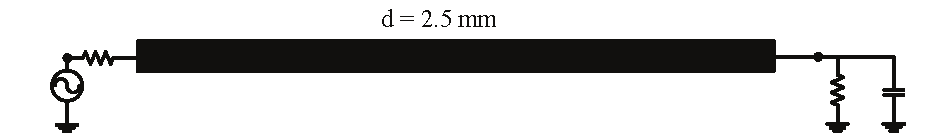
\includegraphics[keepaspectratio=true, width=0.75\textwidth]{TL}
				\caption{Caption goes here.} 
				\label{fig:label}
			\end{figure}    
		\end{verbatim}
	}
\end{SBN}

\begin{figure}[!htp] 
	\centering
	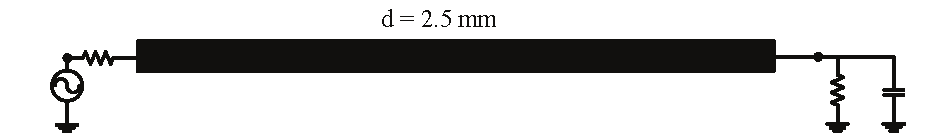
\includegraphics[keepaspectratio=true, width=0.75\textwidth]{TL}
	\caption{Caption goes here.}
	\label{fig:0}
\end{figure} 


%%%%%%%%%%%%%%%%%%%%%%%%%%%%
\subsection{Trimming/Scaling the picture}

\begin{SBN}
{\color{blue}
	\begin{verbatim}
		\begin{figure}[!htp] 
			\centering
			\includegraphics[trim=0in 0in 0in 0in, clip=true, keepaspectratio=true, 
			width=10pc]{universe.jpg}
			\caption{The caption goes here.} 
			\label{fig:label}
		\end{figure}   
	\end{verbatim} 
}
\end{SBN}

\begin{figure}[!ht] 
	\centering
	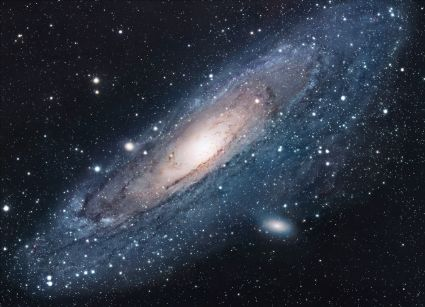
\includegraphics[trim=0in 0in 0in 0in, clip=true, keepaspectratio=true, width=10pc]{uv.jpg}
	\caption{The caption goes here.} 
	\label{fig:1}
\end{figure}


%%%%%%%%%%%%%%%%%%%%%%%%%%%%
\subsection{Figures side-by-side}

\begin{SBN}
\color{blue}
\begin{verbatim}
\begin{figure}[!htp] 
	\centering
	\includegraphics[trim=0in 0in 0in 0in, clip=true,keepaspectratio=true, 
	width=0.75\textwidth]{Graph}
	\includegraphics[trim=0in 0in 0in 0in, clip=true,keepaspectratio=true, 
	width=0.75\textwidth]{universe}
	\caption{\label{fig:label}Caption goes here.} 
\end{figure}    
\end{verbatim}
\end{SBN}


\medskip
\begin{figure}[!htp] 
	\centering
	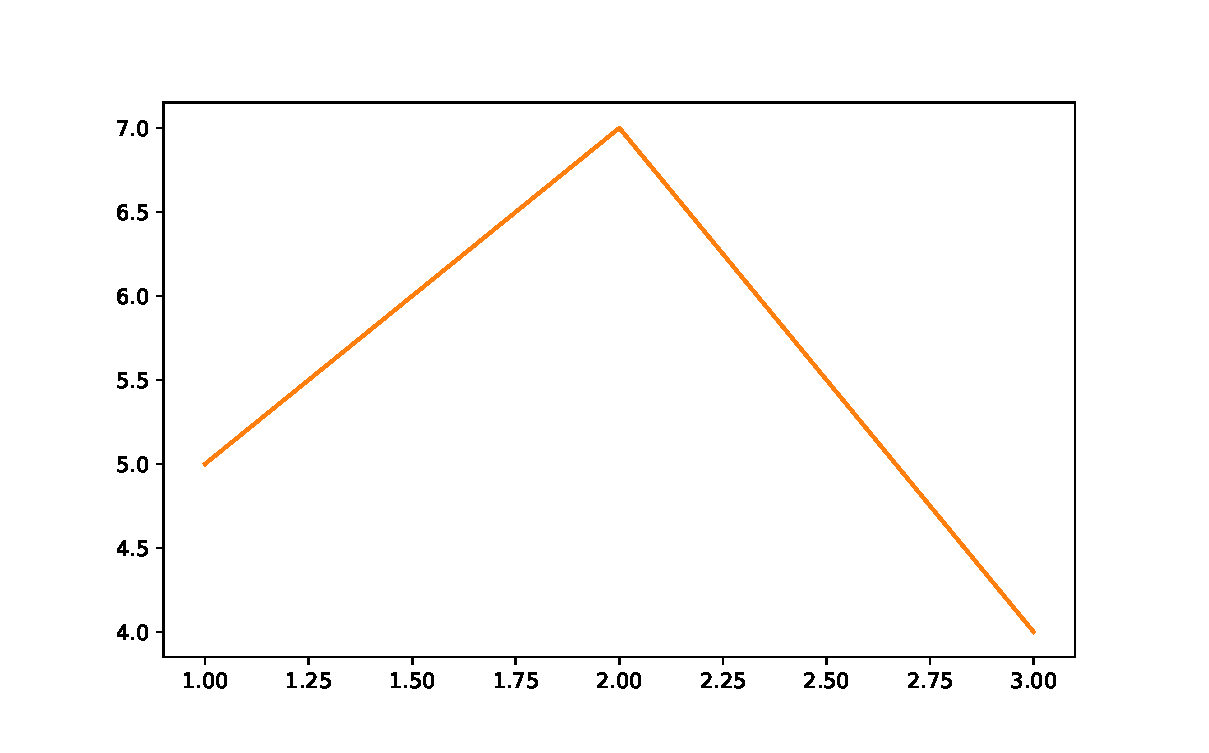
\includegraphics[trim=0in 0.3in 0in 0in, clip=true, keepaspectratio=true, width=.5\textwidth]{f1}
	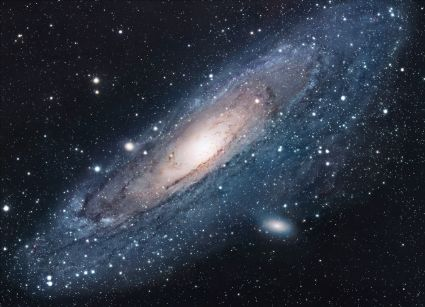
\includegraphics[trim=0in 0in 0in 0in, clip=true, keepaspectratio=true, width=.35\textwidth]{uv.jpg}
	\caption{\label{fig:1000}Caption goes here.}
	
\end{figure} 


%%%%%%%%%%%%%%%%%%%%%%%%%%%%
\subsection{\textbackslash{}infig\{\}}
\begin{SBN}
{\color{blue}\verb!\centerline{\infig{21pc}{smile}{Caption.}}!}
\end{SBN}
\ara{\infig{5pc}{smile}{Caption.}}

\np
\subsubsection{Example: Figure counter}
\begin{SBN}
    {\color{blue}
    \begin{verbatim}
    	\begin{center}
    		\singlespacing
    		\infig{15pc}{smile}{Caption1.}
    		\stepcounter{figure}
    		\includegraphics[width=21pc]{MatlabLogo}
    		\ara{Figure~\arabic{figure}: Caption2.}
    	\end{center}
    \end{verbatim}
    }
\end{SBN}
\bigskip
\begin{center}
	\singlespacing
        \infig{5pc}{\xfigPath/smile}{Caption1.}
	\vspace*{24pt}
	\stepcounter{figure}
	
\includegraphics[width=6pc]{\xfigPath/mat}
	\ara{Figure~\arabic{figure}: Caption2.}
\end{center}


\np
\mypart{Math env.}
%%%%%%%%%%%%%%%%%%%%%%%%%%%%%%%
%%%%%%     Section:      %%%%%%
%%%%%%%%%%%%%%%%%%%%%%%%%%%%%%%
\section{Math equations} \label{sec:math-env}

%%%%%%%%%%%%%%%%%%%%%%%%%%%%
\subsection{Some math symbols} 
\label{sec:math-sym}
%
%
\begin{singlespace}
	\begin{flushleft}
		\begin{longtable}{p{.25\textwidth}p{.6\textwidth}}
			%------------------------------------------------------------
			\verb!x\p!:& $x\p$\\
			\verb!\mat{A}\T!:& $\mat{A}\T$\\
			\verb!\mat{A}\Trans!:& $\mat{A}\Trans$\\
			\verb!\mat{A}\H!:& $\mat{A}\H$\\
			\verb!\mat{A}\Hes!:& $\mat{A}\Hes$\\
			\verb!\mat{A}\NegT!:& $\mat{A}\NegT$\\
			%------------------------------------------------------------
		\end{longtable} 
	\end{flushleft}
\end{singlespace}


%%%%%%%%%%%%%%%%%%%%%%%%%%%%
\section{Equation}

\begin{subnumcases}{\Psi\,:\;}
C\frac{d}{{dt}}x(t)\; + \;Gx(t)\; = \;B\mathbf{u}(t)
\label{t3_a}\\
\mathbf{i}(t)\; = \;\mathbf{L}x(t)\,,
\label{t3_b}
\end{subnumcases}

\begin{verbatim}
\begin{subnumcases}{\label{x} \Psi\,:\;}
C\frac{d}{{dt}}x(t)\; + \;Gx(t)\; = \;B\mathbf{u}(t) \label{x_a}\\
\mathbf{i}(t)\; = \;\mathbf{L}x(t)\,,  \label{x_b}
\end{subnumcases}
\end{verbatim}

\begin{SBN}
\color{blue}
\begin{verbatim}
\begin{equation}
	\label{eq:art1}
	\boxed{	
	\mat{A}=\left[
	\begin{array}{c|cc}
		1 &-2 & 3 \\\hline
		-4 & 5 & 6 \\
		7 & 8 &-9
	\end{array} 
	\right]
	}
\end{equation}
\end{verbatim}
\end{SBN}

\begin{equation}
	\label{eq:art1b}
	\boxed{
	\mat{A}=\left[
	\begin{array}{c|cc}
		1 &-2 & 3 \\\hline
		-4 & 5 & 6 \\
		7 & 8 &-9
	\end{array} 
	\right]
	}
\end{equation}


Let us include an inline equation $x=2$ or a bigger equation in the file. We will refer to it as \eqref{eq:art1b}.

\begin{SBN}
	\begin{verbatim}
		\begin{equation}
			\label{eq:art1c}
			\mat{A}=\left[
			\begin{array}{ccc}
				1 &-2 & 3 \\
				-4 & 5 & 6 \\
				7 & 8 &-9
			\end{array} 
			\right]
		\end{equation}
	\end{verbatim}
	\medskip
	\begin{equation}
		\label{eq:art1d}
		\mat{A}=\left[
		\begin{array}{ccc}
			1 &-2 & 3 \\
			-4 & 5 & 6 \\
			7 & 8 &-9
		\end{array} 
		\right]
	\end{equation}
\end{SBN}
%
%
One may want to do some fancy stuff (e.g.) as shown in \eqref{eq:art2}.
%
\begin{SBN}
	\begin{verbatim}
		\begin{equation}
			\label{eq:art2}
			\mat{A}=\left[
			\begin{array}{c|c|c}
				1 &-2 & 3 \\
				\hline
				-4 & 5 & 6 \\
				\hline
				7 & 8 &-9
			\end{array} 
			\right]
		\end{equation}
	\end{verbatim}
	\medskip
	\begin{equation}
		\label{eq:art2}
		\mat{A}=\left[
		\begin{array}{c|c|c}
			1 &-2 & 3 \\
			\hline
			-4 & 5 & 6 \\
			\hline
			7 & 8 &-9
		\end{array} 
		\right]
	\end{equation}
\end{SBN}
%
%
If an equation is too big to be written in one line We also can split it in two or more lines as shown in \eqref{eq:art3}.
%
%
\begin{SBN}
	\begin{verbatim}
		\begin{multline}
			\label{eq:art3}
			x=q+w+E+r+t+y+u+i+O+p+a+S+D+F+G+H+j+k+l= \\
			SSSSS+L_{11}\times lllll\times (zxc*vbn)^3/2
		\end{multline}
	\end{verbatim}
	\medskip
	\begin{multline}
		\label{eq:art3}
		x=q+w+E+r+t+y+u+i+O+p+a+S+D+F+G+H+j+k+l= \\
		SSSSS+L_{11}\times lllll\times (zxc*vbn)^3/2
	\end{multline}
\end{SBN}
%
May be there are formulas or equations that may look better if the are written in two lines or more as 
%
%
\begin{SBN}
	\begin{verbatim}
		\begin{align}
			\label{eq:art4}
			x &= A+b+C \nonumber  \\
			&= \pm Y^{10}_{ex}  \\
			&= z
		\end{align}
	\end{verbatim}
	\medskip
	\begin{align}
		\label{eq:art4}
		x &= A+b+C \nonumber  \\
		&= \pm Y^{10}_{ex}  \\
		&= z
	\end{align}
\end{SBN}

%
%
The following is sample of a bit twisted way of including an equation.
%
\begin{SBN}
	\begin{verbatim}
		\begin{equation} \label{eq:art10}
			\begin{array}{*{20}{c}}
				\begin{array}{l}
					\textnormal{Error\;in}\\
					\textnormal{Trajectories}\;{\buildrel \Delta \over =}
				\end{array}
				\sqrt{\dfrac{\sum\limits_{j = 1}^N \; \sum\limits_{i = 1}^n 
						{\left({x_i^{(org)}(j)-x_i^{(mor)}(j)}\right)}^2}{n\times N}}
			\end{array}
		\end{equation}
	\end{verbatim}
	\medskip
	\begin{equation} \label{eq:art10}
		\begin{array}{*{20}{c}}
			\begin{array}{l}
				\textnormal{Error\;in}\\
				\textnormal{Trajectories}\;{\buildrel \Delta \over =}
			\end{array}
			\sqrt{\dfrac{\sum\limits_{j = 1}^N \; \sum\limits_{i = 1}^n {\left( {x_i^{(org)}(j)-x_i^{(mor)}(j)} \right)}^2}{n \times N}}
		\end{array}
	\end{equation}
\end{SBN}
%
%

\np
\mypart{Tabular env.}

%%%%%%%%%%%%%%%%%%%%%%%%%%%%%%%
%%%%%%     Section:      %%%%%%
%%%%%%%%%%%%%%%%%%%%%%%%%%%%%%%
\section{Table}

%%%%%%%%%%%%%%%%%%%%%%%%%%%%%%%
\subsection{Sample of \texttt{Table} environment:}
%%%%%%%%%%%%%%%%%%%%%%
\begin{SBN}
\color{blue}
\begin{verbatim}
\begin{table}[!ht]
\caption{Note} 
\centering
 \renewcommand{\arraystretch}{2}
\begin{tabular}{ll} 
\hline
\textbf{Name}   &   \textbf{Definition}\\ 
\hline 
\hline \\
 &  \\
 \multicolumn{2}{l}{spans over two columns}
\end{tabular}
\label{tab:lable}
\end{table}
\end{verbatim}
\end{SBN}
%%%%%%%%%%%%%%%%%%%%%%%%



%%%%%%%%%%%%%%%%%%%%%%%%%%%%%%%
\subsection{Sample 1: \texttt{tabular} env.:}

%%%%%%%%%%%%%%%%%%%%%%
\begin{SBN}
\color{blue}
\begin{verbatim}
\begin{center}
\begin{tabular}{lll | lll| lll}
$\alpha$& \verb!\alpha!& Alpha &
$\beta$& \verb!\beta!& Beta &
$\gamma$& \verb!\gamma!& Gamma \\
\end{tabular}
\end{center}    
\end{verbatim}
\end{SBN}
%%%%%%%%%%%%%%%%%%%%%%%%

\begin{center}
\begin{tabular}{lll | lll| lll}
$\alpha$& \verb!\alpha!& Alpha &
$\beta$& \verb!\beta!& Beta &
$\gamma$& \verb!\gamma!& Gamma \\
\end{tabular}
\end{center}

\vspace*{\baselineskip}
%%%%%%%%%%%%%%%%%%%%%%%%%%%%%%%
\subsection{Sample 2: Simple Table}


%%%%%%%%%%%%%%%%%%%%%
\begin{SBN}
\color{blue}
\begin{verbatim}
\begin{center}
\begin{tabularx}{0.9\textwidth}{ |l|X| }
  \hline
   &  \\ 
  \hline
\end{tabularx}
\end{center}
\end{verbatim}
\end{SBN}
%%%%%%%%%%%%%%%%%%%%

\begin{flushleft}
		\begin{tabularx}{0.9\textwidth}{ |l|X| }
			\hline
			\texttt{optimize}& In compilation process g++ optimizes the build for the speed of running.If you tell it to build optimize, it will make the binary run as fast as
			possible but it will remove all information required for debugging.\\
			\hline   
			\texttt{debug}
			&To compile binary for debugging.\\
			\hline
		\end{tabularx}
\end{flushleft}


\vspace*{\baselineskip}
%%%%%%%%%%%%%%%%%%%%%%%%%%%%%%%
\subsection{Sample 3: Column with prescribed width}


%%%%%%%%%%%%%%%%%%%%%%%%%%%%%%%
\begin{SBN}
\color{blue}
\begin{verbatim}
\begin{center}
\begin{tabularx}{\textwidth}{ |l|p{3cm}|X| }
  \hline
   &  &  \\ 
  \hline
\end{tabularx}
\end{center}
\end{verbatim}
\end{SBN}
%%%%%%%%%%%%%%%%%%%%%%%%%%%%%%


\begin{center}
\begin{tabularx}{\textwidth}{ |l|p{3cm}|X| }
  \hline
  \#1 & This is a Test. This is a Test. & Test title.   \\ \hline
  \#2 & Line-2 & \lipsum[2]\\
  \hline
\end{tabularx}
\end{center}

\vspace*{\baselineskip}
%%%%%%%%%%%%%%%%%%%%%%%%%%%%%%%
\subsection{Sample 4: p,m and b columns in tables}
Source: \url{https://tex.stackexchange.com/questions/35293/p-m-and-b-columns-in-tables}
\begin{SBN}
\color{blue}
\begin{verbatim}
\begin{tabular}{|p{0.3\linewidth}|m{0.3\linewidth}|b{0.3\linewidth}|}
\hline
\centering  &  \centering &  \centering  \tabularnewline
\hline
 &  & 
\tabularnewline
\hline
\end{tabular}
\end{verbatim}
\end{SBN}

\begin{center}
\begin{tabular}{|p{0.22\linewidth}|m{0.22\linewidth}|b{0.22\linewidth}|}
\hline
\centering header p &
\centering header m &   
\centering header b \tabularnewline
\hline
text which is considerably longer than the width of the column& 
text which is considerably longer than the width of the column& 
text which is considerably longer than the width of the column \tabularnewline
\hline
\end{tabular}
\end{center}

\begin{itemize}\packed
\item \textbf{p} means normal cells, they are like parbox with alignment at the top line
\item \textbf{m} means alignment in the vertical center, i.e. the baseline is in the center.
\item \textbf{b} means alignment at the bottom, so the baseline is at the bottom line
\end{itemize}

\begin{figure}[!htp] 
	\centering
	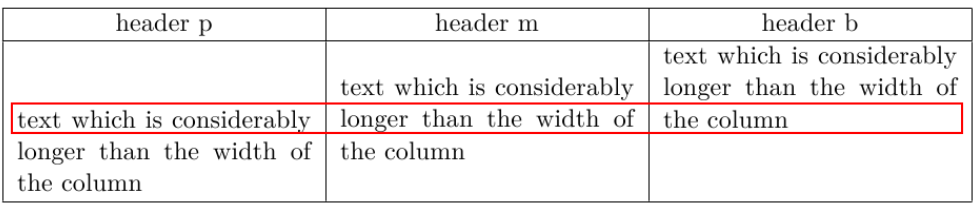
\includegraphics[trim=0in 0in 0in 0in, clip=true,
	keepaspectratio=true, width=0.74\textwidth]{table.png}
	\caption{\label{fig:100}the top line of the first text, the middle of the second and the bottom line of the last text are all in a line.} 
\end{figure}    


\bigskip
%%%%%%%%%%%%%%%%%%%%%%%%%%%%%%%
\subsection{More table examples} \label{app:more-table-examples}

\begin{SBN}
	\begin{verbatim}
		\begin{center}
			\singlespacing\packed
			\begin{tabular}{|c|c|c|c|c|c|}
				\hline
				1& 2 &  3& 4 & 5 & 6 \\
				\hline
				a& b & c & d & e & f \\
				\hline
			\end{tabular}
		\end{center}
	\end{verbatim}
\end{SBN}
\medskip
\begin{center}
	\singlespacing\packed
	\begin{tabular}{|c|c|c|c|c|c|}
		\hline
		1& 2 &  3& 4 & 5 & 6 \\
		\hline
		a& b & c & d & e & f \\
		\hline
	\end{tabular}
\end{center}


\begin{comment}
	This is an example of a table, we refer to as \Table{tab:1}.
	\begin{SBN}
		\begin{verbatim}
			\begin{singlespace}
				\begin{table}[!th]
					\centering  
					\begin{tabular}{|c|c|}
						\hline
						{Use in Netlist}   & {Description} \\ \hline
						\textbf{fs}        & femtosecond   \\ \hline
						\textbf{ps}        & picosecond    \\ \hline
					\end{tabular}
					\caption{Sample table.}
					\label{tab:1}
				\end{table}
			\end{singlespace}
		\end{verbatim}
	\end{SBN}
	
	\medskip
	\begin{singlespace}
		\begin{table}[!th]
			\centering  
			\begin{tabular}{|c|c|}
				\hline
				{Use in Netlist}   & {Description} \\ \hline
				\textbf{fs}        & femtosecond   \\ \hline
				\textbf{ps}        & picosecond    \\ \hline
			\end{tabular}
			\caption{Sample table.}
			\label{tab:1}
		\end{table}
	\end{singlespace}
\end{comment}

\begin{SBN}
	\begin{verbatim}
		\begin{singlespace}
			\begin{table}[!th]
				\centering  
				\begin{tabular}{|c|p{4cm}|}
					\hline
					\textbf{First} & This is a Test. This is a Test. 
					This is a Test. This is a Test. This is a Test. 
					This is a Test. This is a Test.   \\ \hline
				\end{tabular}
				\caption{Sample table.}
				\label{tab:3}
			\end{table}
		\end{singlespace}    
	\end{verbatim}
\end{SBN}

\begin{singlespace}
	\begin{table}[!th]
		\centering  
		\begin{tabular}{|c|p{4cm}|}
			\hline
			\textbf{First} & This is a Test. This is a Test. This is a Test. This is a Test. This is a Test. This is a Test. This is a Test.   \\ \hline
		\end{tabular}
		\caption{Sample table.}
		\label{tab:3}
	\end{table}
\end{singlespace}


%%%%%%%%%%%%%%%%%%%%%%%%%%%%%%%
\subsubsection{\texttt{\textbackslash tabularx}}

\begin{SBN}
	\begin{verbatim}
		\begin{center}
			\begin{tabularx}{\textwidth}{ |l|c|r|X| }
				\hline
				label 1 & label 2 & label 3 & label 4 label 4 
				label 4 label 4 label 4 label 4 \\  \hline 
				item 1 item 1  & item 2 item 2 & item 3 item 3 
				& item 4 item 4 item 4 item 4 item 4 item 4 item 4 
				item 4 \\ \hline
			\end{tabularx} 
		\end{center}
	\end{verbatim}
\end{SBN}


\bigskip
\begin{center}
	\begin{tabularx}{\textwidth}{ |l|c|r|X| }
		\hline
		label 1 & label 2 & label 3 & label 4 label 4 label 4 label 4 label 4 label 4 \\
		\hline 
		item 1 item 1  & item 2 item 2 & item 3 item 3 & item 4 item 4 item 4 item 4 item 4 item 4 item 4 item 4 \\
		\hline
	\end{tabularx}
\end{center}

\vspace*{2\baselineskip}
\begin{SBN}
	\begin{verbatim}
		\begin{center}
			\begin{tabularx}{\textwidth}{ |l|X| }
				\hline
				label 1 & This is a Test. This is a Test. This is a Test. 
				This is a Test. This is a Test. This is a Test. 
				This is a Test.  \\ \hline
			\end{tabularx}
		\end{center}
	\end{verbatim}
\end{SBN}
\medskip
\begin{center}
	\begin{tabularx}{\textwidth}{ |l|X| }
		\hline
		label 1 & This is a Test. This is a Test. This is a Test. This is a Test. This is a Test. This is a Test. This is a Test.  \\
		\hline
	\end{tabularx}
\end{center}


%\vspace*{2\baselineskip}
\np
%%%%%%%%%%%%%%%%%%%%%%%%%%%%%%%
%%%%%%     Appendix      %%%%%%
%%%%%%%%%%%%%%%%%%%%%%%%%%%%%%%
\appendix
\section{Appendix: Sample} \label{app:sample}
\noindent Introduction about \REG{MATLAB} is presented in \App{app:matlab}. 

\bigskip
%%%%%%%%%%%%%%%%%%%%%%%%%%%%
%%%%%%    Section:    %%%%%%
%%%%%%%%%%%%%%%%%%%%%%%%%%%%
\section{Appendix: MATLAB} \label{app:matlab}

\begin{singlespace}
	\lstinputlisting[language=matlab]{\xfigPath/res.m}
\end{singlespace}

\np
%%%%%%%%%%%%%%%%%%%%%%%%%%%%%%%
%%%%%%      Section      %%%%%%
%%%%%%%%%%%%%%%%%%%%%%%%%%%%%%%
\section{Appendix: Using \texttt{BNsh2.sty} package} \label{sec:bnsh2.sty}
\task \verb!\task!
\well \verb!\well!
\bigskip
\todo \verb!\todo!
\done \verb!\done!
\bigskip
\nl \cmark~\verb!\cmark!
\nl \xmark~\verb!\xmark!

%%%%%%%%%%%%%%%%%%%%%%%%%%%%%%%
\subsection{Address symbols}  \label{sec:address}
\begin{tabular}{lll|lll|lll|lll}
\mail & \verb!\mail!  && 
\call & \verb!\call!  &&
\tel  & \verb!\tel!   &&
\phone& \verb!\phone! &\\
\end{tabular}


%%%%%%%%%%%%%%%%%%%%%%%%%%%%%%%
\subsection{Fancy symbols}  \label{sec:fancy-symbols}
\begin{tabular}{lll|lll|lll|lll|lll}
\coffee & \verb!\coffee!  && 
\rest   & \verb!\rest!    &&
\book   & \verb!\book!    &&
\read   & \verb!\read!    &&
\bed    & \verb!\bed!     &\\
\end{tabular}

\bigskip
\begin{tabular}{lll|lll|lll|lll|lll}
\ONEF    & \verb!\ONEF!  && 
\TWOF    & \verb!\TWOF!  &&
\THREEF  & \verb!\THREEF!&&
\FOURF   & \verb!\FOURF! &&
\FIVEF   & \verb!\FIVEF! &\\
\SIXF    & \verb!\SIXF!  && 
\SEVENF  & \verb!\SEVENF!&&
\EIGHTF  & \verb!\EIGHTF!&&
\NINEF   & \verb!\NINEF! &&
\TENF    & \verb!\TENF!  &\\
\end{tabular}

\bigskip
\begin{tabular}{lll|lll|lll|lll|lll}
\ONE    & \verb!\ONE!  && 
\TWO    & \verb!\TWO!  &&
\THREE  & \verb!\THREE!&&
\FOUR   & \verb!\FOUR! &&
\FIVE   & \verb!\FIVE! &\\
\SIX    & \verb!\SIX!  && 
\SEVEN  & \verb!\SEVEN!&&
\EIGHT  & \verb!\EIGHT!&&
\NINE   & \verb!\NINE! &&
\TEN    & \verb!\TEN!  &\\
\end{tabular}


\np
%%%%%%%%%%%%%%%%%%%%%%%%%%%%
%%%%%%    Section:    %%%%%%
%%%%%%%%%%%%%%%%%%%%%%%%%%%%
\section{Appendix: For Defs check \texttt{BNsh2.txt}} \label{sec:bnsh3.sty}
%%%%%%%%%%%%%%%%%%%%%%%%%%%%
\subsection{Address Info}
\subsubsection{Special Symbols of Address, email, etc.} 
 Requires the inclusion of the following font package and some definitions in the preamble:
\begin{SBN}
\begin{verbatim}
\usepackage{fontawesome}
\definecolor{myblue}{RGB}{29,57,127}
\newcommand{\SYM}[1]{\textcolor{myblue}{\csname #1\endcsname}}
\end{verbatim}
\end{SBN}
Then we can have

\begin{SBN}
\begin{verbatim}
\begin{gbox}
	\begin{tabular}{c@{~}l@{~}l}
		\SYM{faAt}             & Email:    & \href{mailto:xxx@ieee.org}{xxx@ieee}\\
		\SYM{email}            & Email:    & \href{mailto: }{ }\\
		\SYM{faMobilePhone}    & Mobile:   & (+1)~xxx~xxx~xxxx\\
		\SYM{faPhone}          & Phone:    & (+1)~xxx~xxx~xxxx\\
		\SYM{tel}              & Phone:    & (+1)~xxx~xxx~xxxx\\	
		\SYM{faMapMarker}      & Address:  & xx Street,\\
		                       &           & City, State, Country~~[pcode]\\
		\SYM{faChain}          & Website:  & \url{www.bnouri.com}\\
		\SYM{faLinkedinSquare} & LinkedIn: & \url{www.bnouri.com} \\
		\SYM{faSkype}          & Skype:    & \texttt{live:sbn\_16}\\
		\SYM{faComment}        & IM:       & live:sbn\_16
	\end{tabular}
\end{gbox}
\end{verbatim}
\end{SBN}

\begin{SBN}
	\begin{tabular}{c@{~}l@{~}l}
		\SYM{faAt}             & Email:    & \href{mailto:xxx@ieee.org}{xxx@ieee}\\
		\SYM{email}            & Email:    & \href{mailto:xxx@ieee.org}{xxx@ieee}\\
		\SYM{faMobilePhone}    & Mobile:   & (+1)~xxx~xxx~xxxx\\
		\SYM{faPhone}          & Phone:    & (+1)~xxx~xxx~xxxx\\
		\SYM{tel}              & Phone:    & (+1)~xxx~xxx~xxxx\\	
		\SYM{faMapMarker}      & Address:  & xx Street,\\
		                       &           & City, State, Country~~[pcode]\\
		\SYM{faChain}          & Website:  & \url{www.bnouri.com}\\
		\SYM{faLinkedinSquare} & LinkedIn: & \url{www.bnouri.com} \\
		\SYM{faSkype}          & Skype:    & \texttt{live:sbn\_16}\\
		\SYM{faComment}        & IM:       & live:sbn\_16
	\end{tabular}
\end{SBN}


\vfill
\begin{SBN}
    \verb!\addPdfdoc{Appendix: Sample for including PDF file}{\xfigPath/pdf2.pdf}!
\end{SBN}
%%%%%%%%%%%%%%%%%%%%%%%%%%%%
%%%%%%    Section:    %%%%%%
%%%%%%%%%%%%%%%%%%%%%%%%%%%%
\addPdfdoc{Appendix: Sample for including PDF file}{\xfigPath/pdf2.pdf}


\nl For more information \cite{ref1,ref2,ref3,ref4} can be also referred to.


\inhand
%%%%%%%%%%%%%%%%%%%%%%%%%%%%%%%
%%%%%%     References    %%%%%%
%%%%%%%%%%%%%%%%%%%%%%%%%%%%%%%
\bibliography{\bibPath/Ref}

%%-- Or alternatively:
%%%%%%%%%%%%%%%%%%%%%%%%%%%%%%%
%%%%%%     References    %%%%%%
%%%%%%%%%%%%%%%%%%%%%%%%%%%%%%%
\begin{comment}
\nl Or equivalently can be used as: \cite{ref1b,ref2b,ref3b,ref4b}
\begin{thebibliography}{1}
\bibitem{ref1b}
A.~Author11 and B.~Author12, ``Jnl paper title,'' \emph{{IEEE} Trans. Microw. Theory Tech.}, pp. 1--10, May 2020.

\bibitem{ref2b}
A.~Author21 and B.~Author22, ``Cnf paper title,'' in \emph{Proc.~xxth {IEEE}
	Conf.}, vol.~1, no.~2, NY, NY, USA, Jan. 2020, pp. 11--22.

\bibitem{ref3b}
A.~Author31, B.~Author32, C.~Author33, and D.~Author34, \emph{Book title},
3rd~ed., ser. Mathematics.\hskip 1em plus 0.5em minus 0.4em\relax City,
State, Country: Father and Son Co., 2022, vol.~II.

\bibitem{ref4b}
A.~Author41 and B.~Author42, \emph{Book Title}, 2nd~ed., ser. Physics.\hskip
1em plus 0.5em minus 0.4em\relax City, State, Country: publisher, 2022,
vol.~IV, ch. Chapter Title, pp. 100--120.
\end{thebibliography}

\end{comment}



\vfill
%%EoF
